\chapter{Flujos y cortes}

En este capítulo, nos centraremos en los siguientes
dos problemas:

\begin{itemize}
\item \key{Encontrar un flujo máximo}:
¿Cuál es la cantidad máxima de flujo que podemos
enviar de un nodo a otro nodo?
\item \key{Encontrar un corte mínimo}:
¿Cuál es un conjunto de aristas de peso mínimo
que separa dos nodos del grafo?
\end{itemize}

La entrada para ambos problemas es un grafo dirigido,
con pesos que contiene dos nodos especiales:
la \emph{fuente} es un nodo sin aristas entrantes,
y el \emph{sumidero} es un nodo sin aristas salientes.

Como ejemplo, usaremos el siguiente grafo
donde el nodo 1 es la fuente y el nodo 6
es el sumidero:

\begin{center}
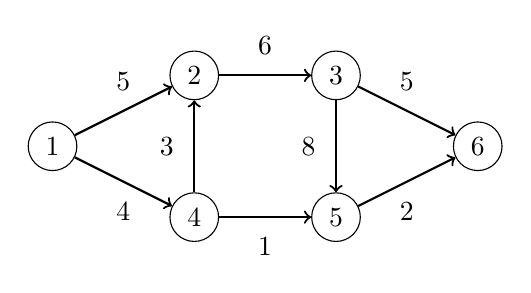
\begin{tikzpicture}[scale=0.9]
\node[draw, circle] (1) at (1,2) {$1$};
\node[draw, circle] (2) at (3,3) {$2$};
\node[draw, circle] (3) at (5,3) {$3$};
\node[draw, circle] (4) at (7,2) {$6$};
\node[draw, circle] (5) at (3,1) {$4$};
\node[draw, circle] (6) at (5,1) {$5$};
\path[draw,thick,->] (1) -- node[font=\small,label=5] {} (2);
\path[draw,thick,->] (2) -- node[font=\small,label=6] {} (3);
\path[draw,thick,->] (3) -- node[font=\small,label=5] {} (4);
\path[draw,thick,->] (1) -- node[font=\small,label=below:4] {} (5);
\path[draw,thick,->] (5) -- node[font=\small,label=below:1] {} (6);
\path[draw,thick,->] (6) -- node[font=\small,label=below:2] {} (4);
\path[draw,thick,<-] (2) -- node[font=\small,label=left:3] {} (5);
\path[draw,thick,->] (3) -- node[font=\small,label=left:8] {} (6);
\end{tikzpicture}
\end{center}

\subsubsection{Flujo máximo}

\index{flujo}
\index{flujo máximo}

En el problema del \key{flujo máximo},
nuestra tarea es enviar la mayor cantidad de flujo posible
de la fuente al sumidero.
El peso de cada arista es una capacidad que
restringe el flujo
que puede pasar por la arista.
En cada nodo intermedio,
el flujo entrante y saliente
tiene que ser igual.

Por ejemplo, el tamaño máximo de un flujo
en el grafo de ejemplo es 7.
La siguiente imagen muestra cómo podemos
enrutar el flujo:

\begin{center}
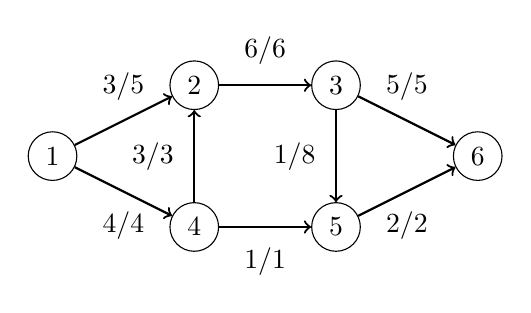
\begin{tikzpicture}[scale=0.9]
\node[draw, circle] (1) at (1,2) {$1$};
\node[draw, circle] (2) at (3,3) {$2$};
\node[draw, circle] (3) at (5,3) {$3$};
\node[draw, circle] (4) at (7,2) {$6$};
\node[draw, circle] (5) at (3,1) {$4$};
\node[draw, circle] (6) at (5,1) {$5$};
\path[draw,thick,->] (1) -- node[font=\small,label=3/5] {} (2);
\path[draw,thick,->] (2) -- node[font=\small,label=6/6] {} (3);
\path[draw,thick,->] (3) -- node[font=\small,label=5/5] {} (4);
\path[draw,thick,->] (1) -- node[font=\small,label=below:4/4] {} (5);
\path[draw,thick,->] (5) -- node[font=\small,label=below:1/1] {} (6);
\path[draw,thick,->] (6) -- node[font=\small,label=below:2/2] {} (4);
\path[draw,thick,<-] (2) -- node[font=\small,label=left:3/3] {} (5);
\path[draw,thick,->] (3) -- node[font=\small,label=left:1/8] {} (6);
\end{tikzpicture}
\end{center}

La notación $v/k$ significa
que se enruta un flujo de $v$ unidades a través de
una arista cuya capacidad es de $k$ unidades.
El tamaño del flujo es $7$,
porque la fuente envía $3+4$ unidades de flujo
y el sumidero recibe $5+2$ unidades de flujo.
Es fácil ver que este flujo es máximo,
porque la capacidad total de las aristas
que conducen al sumidero es $7$.

\subsubsection{Corte mínimo}

\index{corte}
\index{corte mínimo}

En el problema del \key{corte mínimo},
nuestra tarea es eliminar un conjunto
de aristas del grafo
de modo que no haya camino desde la fuente
al sumidero después de la eliminación
y el peso total de las aristas eliminadas
sea mínimo.

El tamaño mínimo de un corte en el grafo de ejemplo es 7.
Basta con eliminar las aristas $2 \rightarrow 3$
y $4 \rightarrow 5$:

\begin{center}
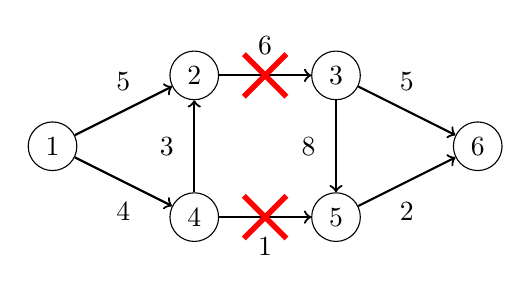
\begin{tikzpicture}[scale=0.9]
\node[draw, circle] (1) at (1,2) {$1$};
\node[draw, circle] (2) at (3,3) {$2$};
\node[draw, circle] (3) at (5,3) {$3$};
\node[draw, circle] (4) at (7,2) {$6$};
\node[draw, circle] (5) at (3,1) {$4$};
\node[draw, circle] (6) at (5,1) {$5$};
\path[draw,thick,->] (1) -- node[font=\small,label=5] {} (2);
\path[draw,thick,->] (2) -- node[font=\small,label=6] {} (3);
\path[draw,thick,->] (3) -- node[font=\small,label=5] {} (4);
\path[draw,thick,->] (1) -- node[font=\small,label=below:4] {} (5);
\path[draw,thick,->] (5) -- node[font=\small,label=below:1] {} (6);
\path[draw,thick,->] (6) -- node[font=\small,label=below:2] {} (4);
\path[draw,thick,<-] (2) -- node[font=\small,label=left:3] {} (5);
\path[draw,thick,->] (3) -- node[font=\small,label=left:8] {} (6);

\path[draw=red,thick,-,line width=2pt] (4-.3,3-.3) -- (4+.3,3+.3);
\path[draw=red,thick,-,line width=2pt] (4-.3,3+.3) -- (4+.3,3-.3);
\path[draw=red,thick,-,line width=2pt] (4-.3,1-.3) -- (4+.3,1+.3);
\path[draw=red,thick,-,line width=2pt] (4-.3,1+.3) -- (4+.3,1-.3);
\end{tikzpicture}
\end{center}


Después de eliminar los bordes,
no habrá ningún camino desde la fuente hasta el sumidero.
El tamaño del corte es $7$,
porque los pesos de los bordes eliminados
son $6$ y $1$.
El corte es mínimo, porque no hay una forma válida
de eliminar bordes del gráfico de modo que
su peso total sea menor que $7$.
\\\\
No es una coincidencia que
el tamaño máximo de un flujo
y el tamaño mínimo de un corte
sean los mismos en el ejemplo anterior.
Resulta que un flujo máximo
y un corte mínimo son
\emph{siempre} igualmente grandes,
por lo que los conceptos son dos caras de la misma moneda.

A continuación, discutiremos el algoritmo de Ford–Fulkerson
que se puede utilizar para encontrar
el flujo máximo y el corte mínimo de un gráfico.
El algoritmo también nos ayuda a entender
\emph{por qué} son igualmente grandes.

\section{Algoritmo de Ford–Fulkerson}

\index{Algoritmo de Ford–Fulkerson}

El \key{algoritmo de Ford–Fulkerson} \cite{for56} encuentra
el flujo máximo en un gráfico.
El algoritmo comienza con un flujo vacío,
y en cada paso encuentra un camino desde la fuente
hasta el sumidero que genera más flujo.
Finalmente, cuando el algoritmo no puede aumentar el flujo
más, se ha encontrado el flujo máximo.

El algoritmo utiliza una representación especial
del gráfico donde cada borde original tiene un inverso
borde en otra dirección.
El peso de cada borde indica cuánta más flujo
podríamos enrutar a través de él.
Al comienzo del algoritmo, el peso de cada borde original
es igual a la capacidad del borde
y el peso de cada borde inverso es cero.

\begin{samepage}
La nueva representación para el gráfico de ejemplo es la siguiente:

\begin{center}
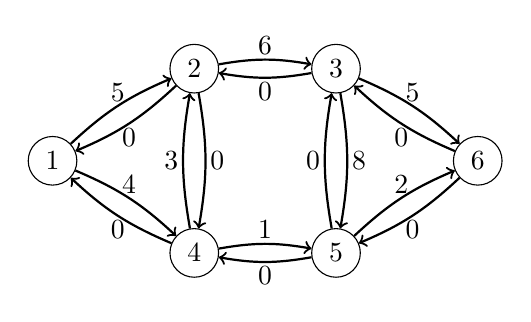
\begin{tikzpicture}[scale=0.9,label distance=-2mm]
\node[draw, circle] (1) at (1,1.3) {$1$};
\node[draw, circle] (2) at (3,2.6) {$2$};
\node[draw, circle] (3) at (5,2.6) {$3$};
\node[draw, circle] (4) at (7,1.3) {$6$};
\node[draw, circle] (5) at (3,0) {$4$};
\node[draw, circle] (6) at (5,0) {$5$};

\path[draw,thick,->] (1) edge [bend left=10] node[font=\small,label=5] {} (2);
\path[draw,thick,->] (2) edge [bend left=10] node[font=\small,label=below:0] {} (1);
\path[draw,thick,->] (2) edge [bend left=10] node[font=\small,label=6] {} (3);
\path[draw,thick,->] (3) edge [bend left=10] node[font=\small,label=below:0] {} (2);
\path[draw,thick,->] (3) edge [bend left=10] node[font=\small,label=5] {} (4);
\path[draw,thick,->] (4) edge [bend left=10] node[font=\small,label=below:0] {} (3);
\path[draw,thick,->] (1) edge [bend left=10] node[font=\small,label=4] {} (5);
\path[draw,thick,->] (5) edge [bend left=10] node[font=\small,label=below:0] {} (1);
\path[draw,thick,->] (5) edge [bend left=10] node[font=\small,label=1] {} (6);
\path[draw,thick,->] (6) edge [bend left=10] node[font=\small,label=below:0] {} (5);
\path[draw,thick,->] (6) edge [bend left=10] node[font=\small,label=2] {} (4);
\path[draw,thick,->] (4) edge [bend left=10] node[font=\small,label=below:0] {} (6);
\path[draw,thick,->] (5) edge [bend left=10] node[font=\small,label=left:3] {} (2);
\path[draw,thick,->] (2) edge [bend left=10] node[font=\small,label=right:0] {} (5);
\path[draw,thick,->] (3) edge [bend left=10] node[font=\small,label=right:8] {} (6);
\path[draw,thick,->] (6) edge [bend left=10] node[font=\small,label=left:0] {} (3);
\end{tikzpicture}
\end{center}
\end{samepage}

\subsubsection{Descripción del algoritmo}

El algoritmo de Ford–Fulkerson consta de varios
rondas.
En cada ronda, el algoritmo encuentra
un camino desde la fuente hasta el sumidero
tal que cada borde en el camino tiene un peso positivo.
Si hay más de un camino posible disponible,
podemos elegir cualquiera de ellos.

Por ejemplo, supongamos que elegimos el siguiente camino:

\begin{center}
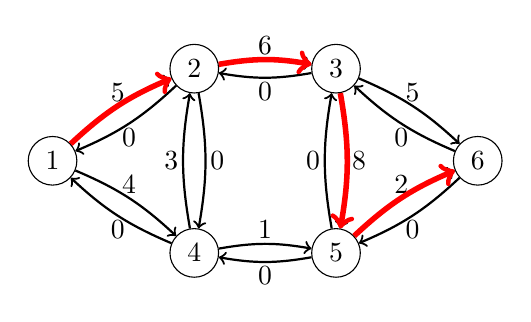
\begin{tikzpicture}[scale=0.9,label distance=-2mm]
\node[draw, circle] (1) at (1,1.3) {$1$};
\node[draw, circle] (2) at (3,2.6) {$2$};
\node[draw, circle] (3) at (5,2.6) {$3$};
\node[draw, circle] (4) at (7,1.3) {$6$};
\node[draw, circle] (5) at (3,0) {$4$};
\node[draw, circle] (6) at (5,0) {$5$};

\path[draw,thick,->] (1) edge [bend left=10] node[font=\small,label=5] {} (2);
\path[draw,thick,->] (2) edge [bend left=10] node[font=\small,label=below:0] {} (1);
\path[draw,thick,->] (2) edge [bend left=10] node[font=\small,label=6] {} (3);
\path[draw,thick,->] (3) edge [bend left=10] node[font=\small,label=below:0] {} (2);
\path[draw,thick,->] (3) edge [bend left=10] node[font=\small,label=5] {} (4);
\path[draw,thick,->] (4) edge [bend left=10] node[font=\small,label=below:0] {} (3);
\path[draw,thick,->] (1) edge [bend left=10] node[font=\small,label=4] {} (5);
\path[draw,thick,->] (5) edge [bend left=10] node[font=\small,label=below:0] {} (1);
\path[draw,thick,->] (5) edge [bend left=10] node[font=\small,label=1] {} (6);
\path[draw,thick,->] (6) edge [bend left=10] node[font=\small,label=below:0] {} (5);
\path[draw,thick,->] (6) edge [bend left=10] node[font=\small,label=2] {} (4);
\path[draw,thick,->] (4) edge [bend left=10] node[font=\small,label=below:0] {} (6);
\path[draw,thick,->] (5) edge [bend left=10] node[font=\small,label=left:3] {} (2);
\path[draw,thick,->] (2) edge [bend left=10] node[font=\small,label=right:0] {} (5);
\path[draw,thick,->] (3) edge [bend left=10] node[font=\small,label=right:8] {} (6);
\path[draw,thick,->] (6) edge [bend left=10] node[font=\small,label=left:0] {} (3);

\path[draw=red,thick,->,line width=2pt] (1) edge [bend left=10] (2);
\path[draw=red,thick,->,line width=2pt] (2) edge [bend left=10] (3);
\path[draw=red,thick,->,line width=2pt] (3) edge [bend left=10] (6);
\path[draw=red,thick,->,line width=2pt] (6) edge [bend left=10] (4);
\end{tikzpicture}
\end{center}

Después de elegir la ruta, el flujo aumenta en $x$ unidades,
donde $x$ es el peso de borde más pequeño en la ruta.
Además, el peso de cada borde en la ruta
disminuye en $x$ y el peso de cada borde inverso
aumenta en $x$.

En la ruta anterior, los pesos de los
bordes son 5, 6, 8 y 2.
El peso más pequeño es 2,
por lo que el flujo aumenta en 2
y el nuevo gráfico es el siguiente:

\begin{center}
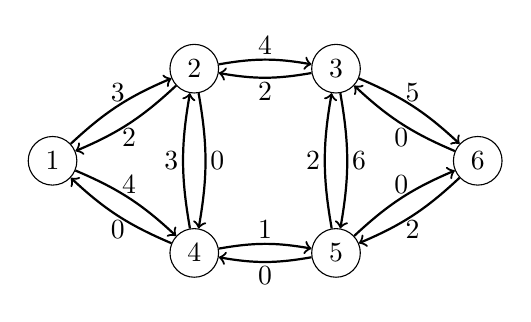
\begin{tikzpicture}[scale=0.9,label distance=-2mm]
\node[draw, circle] (1) at (1,1.3) {$1$};
\node[draw, circle] (2) at (3,2.6) {$2$};
\node[draw, circle] (3) at (5,2.6) {$3$};
\node[draw, circle] (4) at (7,1.3) {$6$};
\node[draw, circle] (5) at (3,0) {$4$};
\node[draw, circle] (6) at (5,0) {$5$};

\path[draw,thick,->] (1) edge [bend left=10] node[font=\small,label=3] {} (2);
\path[draw,thick,->] (2) edge [bend left=10] node[font=\small,label=below:2] {} (1);
\path[draw,thick,->] (2) edge [bend left=10] node[font=\small,label=4] {} (3);
\path[draw,thick,->] (3) edge [bend left=10] node[font=\small,label=below:2] {} (2);
\path[draw,thick,->] (3) edge [bend left=10] node[font=\small,label=5] {} (4);
\path[draw,thick,->] (4) edge [bend left=10] node[font=\small,label=below:0] {} (3);
\path[draw,thick,->] (1) edge [bend left=10] node[font=\small,label=4] {} (5);
\path[draw,thick,->] (5) edge [bend left=10] node[font=\small,label=below:0] {} (1);
\path[draw,thick,->] (5) edge [bend left=10] node[font=\small,label=1] {} (6);
\path[draw,thick,->] (6) edge [bend left=10] node[font=\small,label=below:0] {} (5);
\path[draw,thick,->] (6) edge [bend left=10] node[font=\small,label=0] {} (4);
\path[draw,thick,->] (4) edge [bend left=10] node[font=\small,label=below:2] {} (6);
\path[draw,thick,->] (5) edge [bend left=10] node[font=\small,label=left:3] {} (2);
\path[draw,thick,->] (2) edge [bend left=10] node[font=\small,label=right:0] {} (5);
\path[draw,thick,->] (3) edge [bend left=10] node[font=\small,label=right:6] {} (6);
\path[draw,thick,->] (6) edge [bend left=10] node[font=\small,label=left:2] {} (3);
\end{tikzpicture}
\end{center}

La idea es que aumentar el flujo disminuye la cantidad de
flujo que puede pasar a través de los bordes en el futuro.
Por otro lado, es posible cancelar
el flujo más tarde usando los bordes inversos del gráfico
si resulta que
sería beneficioso enrutar el flujo de otra manera.

El algoritmo aumenta el flujo mientras
exista una ruta desde la fuente
hasta el sumidero a través de bordes de peso positivo.
En el ejemplo actual, nuestra siguiente ruta puede ser la siguiente:

\begin{center}
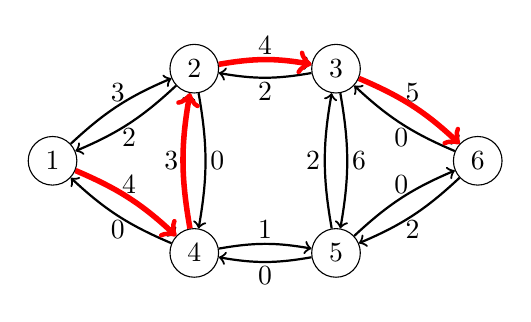
\begin{tikzpicture}[scale=0.9,label distance=-2mm]
\node[draw, circle] (1) at (1,1.3) {$1$};
\node[draw, circle] (2) at (3,2.6) {$2$};
\node[draw, circle] (3) at (5,2.6) {$3$};
\node[draw, circle] (4) at (7,1.3) {$6$};
\node[draw, circle] (5) at (3,0) {$4$};
\node[draw, circle] (6) at (5,0) {$5$};
\path[draw,thick,->] (1) edge [bend left=10] node[font=\small,label=3] {} (2);
\path[draw,thick,->] (2) edge [bend left=10] node[font=\small,label=below:2] {} (1);
\path[draw,thick,->] (2) edge [bend left=10] node[font=\small,label=4] {} (3);
\path[draw,thick,->] (3) edge [bend left=10] node[font=\small,label=below:2] {} (2);
\path[draw,thick,->] (3) edge [bend left=10] node[font=\small,label=5] {} (4);
\path[draw,thick,->] (4) edge [bend left=10] node[font=\small,label=below:0] {} (3);
\path[draw,thick,->] (1) edge [bend left=10] node[font=\small,label=4] {} (5);
\path[draw,thick,->] (5) edge [bend left=10] node[font=\small,label=below:0] {} (1);
\path[draw,thick,->] (5) edge [bend left=10] node[font=\small,label=1] {} (6);
\path[draw,thick,->] (6) edge [bend left=10] node[font=\small,label=below:0] {} (5);
\path[draw,thick,->] (6) edge [bend left=10] node[font=\small,label=0] {} (4);
\path[draw,thick,->] (4) edge [bend left=10] node[font=\small,label=below:2] {} (6);
\path[draw,thick,->] (5) edge [bend left=10] node[font=\small,label=left:3] {} (2);
\path[draw,thick,->] (2) edge [bend left=10] node[font=\small,label=right:0] {} (5);
\path[draw,thick,->] (3) edge [bend left=10] node[font=\small,label=right:6] {} (6);
\path[draw,thick,->] (6) edge [bend left=10] node[font=\small,label=left:2] {} (3);

\path[draw=red,thick,->,line width=2pt] (1) edge [bend left=10] (5);
\path[draw=red,thick,->,line width=2pt] (5) edge [bend left=10] (2);
\path[draw=red,thick,->,line width=2pt] (2) edge [bend left=10] (3);
\path[draw=red,thick,->,line width=2pt] (3) edge [bend left=10] (4);
\end{tikzpicture}
\end{center}

El peso mínimo de la arista en este camino es 3,
por lo que el camino aumenta el flujo en 3,
y el flujo total después de procesar el camino es 5.

\begin{samepage}
El nuevo gráfico será como sigue:

\begin{center}
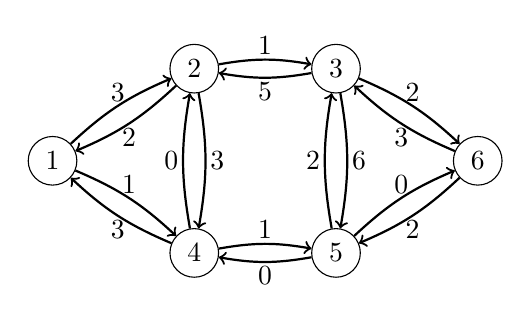
\begin{tikzpicture}[scale=0.9,label distance=-2mm]
\node[draw, circle] (1) at (1,1.3) {$1$};
\node[draw, circle] (2) at (3,2.6) {$2$};
\node[draw, circle] (3) at (5,2.6) {$3$};
\node[draw, circle] (4) at (7,1.3) {$6$};
\node[draw, circle] (5) at (3,0) {$4$};
\node[draw, circle] (6) at (5,0) {$5$};

\path[draw,thick,->] (1) edge [bend left=10] node[font=\small,label=3] {} (2);
\path[draw,thick,->] (2) edge [bend left=10] node[font=\small,label=below:2] {} (1);
\path[draw,thick,->] (2) edge [bend left=10] node[font=\small,label=1] {} (3);
\path[draw,thick,->] (3) edge [bend left=10] node[font=\small,label=below:5] {} (2);
\path[draw,thick,->] (3) edge [bend left=10] node[font=\small,label=2] {} (4);
\path[draw,thick,->] (4) edge [bend left=10] node[font=\small,label=below:3] {} (3);
\path[draw,thick,->] (1) edge [bend left=10] node[font=\small,label=1] {} (5);
\path[draw,thick,->] (5) edge [bend left=10] node[font=\small,label=below:3] {} (1);
\path[draw,thick,->] (5) edge [bend left=10] node[font=\small,label=1] {} (6);
\path[draw,thick,->] (6) edge [bend left=10] node[font=\small,label=below:0] {} (5);
\path[draw,thick,->] (6) edge [bend left=10] node[font=\small,label=0] {} (4);
\path[draw,thick,->] (4) edge [bend left=10] node[font=\small,label=below:2] {} (6);
\path[draw,thick,->] (5) edge [bend left=10] node[font=\small,label=left:0] {} (2);
\path[draw,thick,->] (2) edge [bend left=10] node[font=\small,label=right:3] {} (5);
\path[draw,thick,->] (3) edge [bend left=10] node[font=\small,label=right:6] {} (6);
\path[draw,thick,->] (6) edge [bend left=10] node[font=\small,label=left:2] {} (3);
\end{tikzpicture}
\end{center}
\end{samepage}

Todavía necesitamos dos rondas más antes de alcanzar el flujo máximo.
Por ejemplo, podemos elegir los caminos
$1 \rightarrow 2 \rightarrow 3 \rightarrow 6$ y
$1 \rightarrow 4 \rightarrow 5 \rightarrow 3 \rightarrow 6$.
Ambos caminos aumentan el flujo en 1,
y el gráfico final es como sigue:

\begin{center}
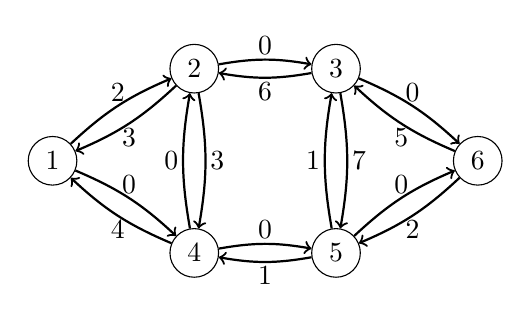
\begin{tikzpicture}[scale=0.9,label distance=-2mm]
\node[draw, circle] (1) at (1,1.3) {$1$};
\node[draw, circle] (2) at (3,2.6) {$2$};
\node[draw, circle] (3) at (5,2.6) {$3$};
\node[draw, circle] (4) at (7,1.3) {$6$};
\node[draw, circle] (5) at (3,0) {$4$};
\node[draw, circle] (6) at (5,0) {$5$};
\path[draw,thick,->] (1) edge [bend left=10] node[font=\small,label=2] {} (2);
\path[draw,thick,->] (2) edge [bend left=10] node[font=\small,label=below:3] {} (1);
\path[draw,thick,->] (2) edge [bend left=10] node[font=\small,label=0] {} (3);
\path[draw,thick,->] (3) edge [bend left=10] node[font=\small,label=below:6] {} (2);
\path[draw,thick,->] (3) edge [bend left=10] node[font=\small,label=0] {} (4);
\path[draw,thick,->] (4) edge [bend left=10] node[font=\small,label=below:5] {} (3);
\path[draw,thick,->] (1) edge [bend left=10] node[font=\small,label=0] {} (5);
\path[draw,thick,->] (5) edge [bend left=10] node[font=\small,label=below:4] {} (1);
\path[draw,thick,->] (5) edge [bend left=10] node[font=\small,label=0] {} (6);
\path[draw,thick,->] (6) edge [bend left=10] node[font=\small,label=below:1] {} (5);
\path[draw,thick,->] (6) edge [bend left=10] node[font=\small,label=0] {} (4);
\path[draw,thick,->] (4) edge [bend left=10] node[font=\small,label=below:2] {} (6);
\path[draw,thick,->] (5) edge [bend left=10] node[font=\small,label=left:0] {} (2);
\path[draw,thick,->] (2) edge [bend left=10] node[font=\small,label=right:3] {} (5);
\path[draw,thick,->] (3) edge [bend left=10] node[font=\small,label=right:7] {} (6);
\path[draw,thick,->] (6) edge [bend left=10] node[font=\small,label=left:1] {} (3);
\end{tikzpicture}
\end{center}

No es posible aumentar el flujo más,
porque no hay camino desde la fuente
al sumidero con pesos de borde positivos.
Por lo tanto, el algoritmo termina y el flujo máximo es 7.

\subsubsection{Encontrar caminos}

El algoritmo de Ford–Fulkerson no especifica
cómo debemos elegir los caminos que aumentan el flujo.
En cualquier caso, el algoritmo terminará tarde o temprano
y encontrará correctamente el flujo máximo.
Sin embargo, la eficiencia del algoritmo depende de
la forma en que se eligen los caminos.

Una forma sencilla de encontrar caminos es usar la búsqueda en profundidad.
Por lo general, esto funciona bien, pero en el peor de los casos,
cada camino solo aumenta el flujo en 1
y el algoritmo es lento.
Afortunadamente, podemos evitar esta situación
utilizando una de las siguientes técnicas:

\index{Algoritmo de Edmonds–Karp}

El \key{algoritmo de Edmonds–Karp} \cite{edm72}
elige cada camino de modo que el número de aristas
en el camino sea lo más pequeño posible.
Esto se puede hacer utilizando la búsqueda en amplitud
en lugar de la búsqueda en profundidad para encontrar caminos.
Se puede probar que esto garantiza que
el flujo aumente rápidamente, y la complejidad temporal
del algoritmo es $O(m^2 n)$.

\index{Algoritmo de escalado}

El \key{algoritmo de escalado} \cite{ahu91} utiliza la búsqueda en profundidad
para encontrar caminos donde cada peso de arista es
al menos un valor umbral.
Inicialmente, el valor umbral es
algún número grande, por ejemplo, la suma de todos
los pesos de arista del gráfico.
Siempre que no se pueda encontrar un camino,
el valor umbral se divide por 2.
La complejidad temporal del algoritmo es $O(m^2 \log c)$,
donde $c$ es el valor umbral inicial.

En la práctica, el algoritmo de escalado es más fácil de implementar,
porque la búsqueda en profundidad se puede utilizar para encontrar caminos.
Ambos algoritmos son lo suficientemente eficientes para problemas
que normalmente aparecen en las competiciones de programación.

\subsubsection{Cortes mínimos}

\index{Corte mínimo}

Resulta que una vez que el algoritmo de Ford–Fulkerson
ha encontrado un flujo máximo,
también ha determinado un corte mínimo.
Sea $A$ el conjunto de nodos
que se pueden alcanzar desde la fuente
usando aristas de peso positivo.
En el gráfico de ejemplo, $A$ contiene los nodos 1, 2 y 4:

\begin{center}
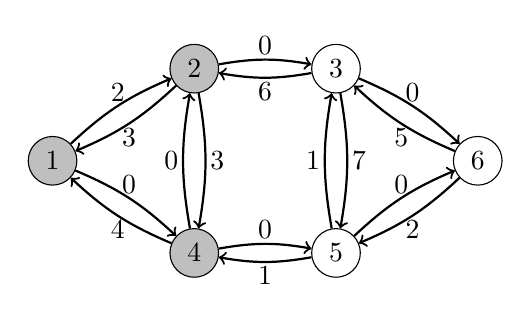
\begin{tikzpicture}[scale=0.9,label distance=-2mm]
\node[draw, circle,fill=lightgray] (1) at (1,1.3) {$1$};
\node[draw, circle,fill=lightgray] (2) at (3,2.6) {$2$};
\node[draw, circle] (3) at (5,2.6) {$3$};
\node[draw, circle] (4) at (7,1.3) {$6$};
\node[draw, circle,fill=lightgray] (5) at (3,0) {$4$};
\node[draw, circle] (6) at (5,0) {$5$};
\path[draw,thick,->] (1) edge [bend left=10] node[font=\small,label=2] {} (2);
\path[draw,thick,->] (2) edge [bend left=10] node[font=\small,label=below:3] {} (1);
\path[draw,thick,->] (2) edge [bend left=10] node[font=\small,label=0] {} (3);
\path[draw,thick,->] (3) edge [bend left=10] node[font=\small,label=below:6] {} (2);
\path[draw,thick,->] (3) edge [bend left=10] node[font=\small,label=0] {} (4);
\path[draw,thick,->] (4) edge [bend left=10] node[font=\small,label=below:5] {} (3);
\path[draw,thick,->] (1) edge [bend left=10] node[font=\small,label=0] {} (5);
\path[draw,thick,->] (5) edge [bend left=10] node[font=\small,label=below:4] {} (1);
\path[draw,thick,->] (5) edge [bend left=10] node[font=\small,label=0] {} (6);
\path[draw,thick,->] (6) edge [bend left=10] node[font=\small,label=below:1] {} (5);
\path[draw,thick,->] (6) edge [bend left=10] node[font=\small,label=0] {} (4);
\path[draw,thick,->] (4) edge [bend left=10] node[font=\small,label=below:2] {} (6);
\path[draw,thick,->] (5) edge [bend left=10] node[font=\small,label=left:0] {} (2);
\path[draw,thick,->] (2) edge [bend left=10] node[font=\small,label=right:3] {} (5);
\path[draw,thick,->] (3) edge [bend left=10] node[font=\small,label=right:7] {} (6);
\path[draw,thick,->] (6) edge [bend left=10] node[font=\small,label=left:1] {} (3);
\end{tikzpicture}
\end{center}

Ahora, el corte mínimo consta de los bordes del gráfico original
que comienzan en algún nodo en $A$, terminan en algún nodo fuera de $A$,
y cuya capacidad se utiliza completamente
en el flujo máximo.
En el gráfico anterior, estos bordes son
$2 \rightarrow 3$ y $4 \rightarrow 5$,
que corresponden al corte mínimo $6+1=7$.

¿Por qué el flujo producido por el algoritmo es máximo
y por qué es el corte mínimo?
La razón es que un gráfico no puede
contener un flujo cuyo tamaño sea mayor
que el peso de cualquier corte del gráfico.
Por lo tanto, siempre que un flujo y un corte son igualmente grandes,
son un flujo máximo y un corte mínimo.

Consideremos cualquier corte del gráfico
tal que la fuente pertenezca a $A$,
el sumidero pertenezca a $B$
y haya algunos bordes entre los conjuntos:

\begin{center}
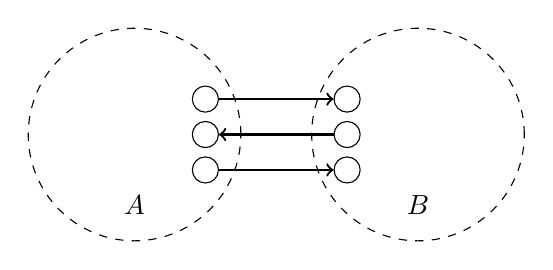
\begin{tikzpicture}[scale=0.9]
\draw[dashed] (-2,0) circle (1.5);
\draw[dashed] (2,0) circle (1.5);

\node at (-2,-1) {$A$};
\node at (2,-1) {$B$};

\node[draw, circle] (1) at (-1,0.5) {};
\node[draw, circle] (2) at (-1,0) {};
\node[draw, circle] (3) at (-1,-0.5) {};
\node[draw, circle] (4) at (1,0.5) {};
\node[draw, circle] (5) at (1,0) {};
\node[draw, circle] (6) at (1,-0.5) {};

\path[draw,thick,->] (1) -- (4);
\path[draw,thick,->] (5) -- (2);
\path[draw,thick,->] (3) -- (6);

\end{tikzpicture}
\end{center}

El tamaño del corte es la suma de los bordes
que van de $A$ a $B$.
Este es un límite superior para el flujo
en el gráfico, porque el flujo tiene que proceder
de $A$ a $B$.
Por lo tanto, el tamaño de un flujo máximo es menor o igual que
el tamaño de cualquier corte en el gráfico.

Por otro lado, el algoritmo de Ford–Fulkerson
produce un flujo cuyo tamaño es \emph{exactamente} tan grande
como el tamaño de un corte en el gráfico.
Por lo tanto, el flujo tiene que ser un flujo máximo
y el corte tiene que ser un corte mínimo.

\section{Caminos disjuntos}

Muchos problemas de gráficos se pueden resolver reduciéndolos
al problema de flujo máximo.
Nuestro primer ejemplo de tal problema es
el siguiente: se nos da un gráfico dirigido
con una fuente y un sumidero,
y nuestra tarea es encontrar el número máximo
de caminos disjuntos desde la fuente hasta el sumidero.

\subsubsection{Caminos disjuntos de borde}

Primero nos centraremos en el problema de
encontrar el número máximo de
\key{caminos disjuntos de borde} desde la fuente hasta el sumidero.
Esto significa que debemos construir un conjunto de caminos
de modo que cada borde aparezca en como máximo un camino.

Por ejemplo, considere el siguiente gráfico:
\begin{center}
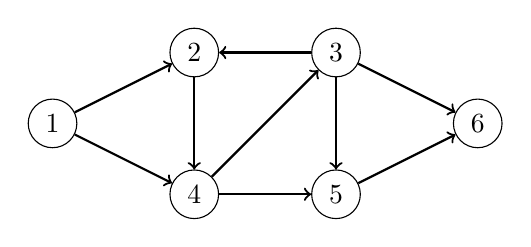
\begin{tikzpicture}[scale=0.9]
\node[draw, circle] (1) at (1,2) {$1$};
\node[draw, circle] (2) at (3,3) {$2$};
\node[draw, circle] (3) at (5,3) {$3$};
\node[draw, circle] (4) at (3,1) {$4$};
\node[draw, circle] (5) at (5,1) {$5$};
\node[draw, circle] (6) at (7,2) {$6$};
\path[draw,thick,->] (1) -- (2);
\path[draw,thick,->] (1) -- (4);
\path[draw,thick,->] (2) -- (4);
\path[draw,thick,->] (3) -- (2);
\path[draw,thick,->] (3) -- (5);
\path[draw,thick,->] (3) -- (6);
\path[draw,thick,->] (4) -- (3);
\path[draw,thick,->] (4) -- (5);
\path[draw,thick,->] (5) -- (6);
\end{tikzpicture}
\end{center}

En este gráfico, el número máximo de caminos disjuntos de borde
es 2.
Podemos elegir los caminos
$1 \rightarrow 2 \rightarrow 4 \rightarrow 3 \rightarrow 6$
y $1 \rightarrow 4 \rightarrow 5 \rightarrow 6$ de la siguiente manera:
\begin{center}
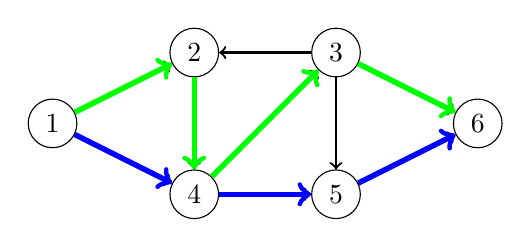
\begin{tikzpicture}[scale=0.9]
\node[draw, circle] (1) at (1,2) {$1$};
\node[draw, circle] (2) at (3,3) {$2$};
\node[draw, circle] (3) at (5,3) {$3$};
\node[draw, circle] (4) at (3,1) {$4$};
\node[draw, circle] (5) at (5,1) {$5$};
\node[draw, circle] (6) at (7,2) {$6$};
\path[draw,thick,->] (1) -- (2);
\path[draw,thick,->] (1) -- (4);
\path[draw,thick,->] (2) -- (4);
\path[draw,thick,->] (3) -- (2);
\path[draw,thick,->] (3) -- (5);
\path[draw,thick,->] (3) -- (6);
\path[draw,thick,->] (4) -- (3);
\path[draw,thick,->] (4) -- (5);
\path[draw,thick,->] (5) -- (6);

\path[draw=green,thick,->,line width=2pt] (1) -- (2);
\path[draw=green,thick,->,line width=2pt] (2) -- (4);
\path[draw=green,thick,->,line width=2pt] (4) -- (3);
\path[draw=green,thick,->,line width=2pt] (3) -- (6);

\path[draw=blue,thick,->,line width=2pt] (1) -- (4);
\path[draw=blue,thick,->,line width=2pt] (4) -- (5);
\path[draw=blue,thick,->,line width=2pt] (5) -- (6);
\end{tikzpicture}
\end{center}

Resulta que el número máximo de
caminos disjuntos de aristas
es igual al flujo máximo del grafo,
asumiendo que la capacidad de cada arista es uno.
Después de que se ha construido el flujo máximo,
los caminos disjuntos de aristas se pueden encontrar codiciosamente
siguiendo caminos desde la fuente hasta el sumidero.

\subsubsection{Caminos disjuntos de nodos}

Consideremos ahora otro problema:
encontrar el número máximo de
\key{caminos disjuntos de nodos} desde la fuente
hasta el sumidero.
En este problema, cada nodo,
excepto la fuente y el sumidero,
puede aparecer en como máximo un camino.
El número de caminos disjuntos de nodos
puede ser menor que el número de
caminos disjuntos de aristas.

Por ejemplo, en el gráfico anterior,
el número máximo de caminos disjuntos de nodos es 1:

\begin{center}
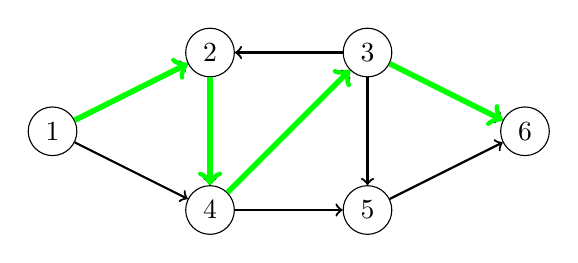
\begin{tikzpicture}
\node[draw, circle] (1) at (1,2) {$1$};
\node[draw, circle] (2) at (3,3) {$2$};
\node[draw, circle] (3) at (5,3) {$3$};
\node[draw, circle] (4) at (3,1) {$4$};
\node[draw, circle] (5) at (5,1) {$5$};
\node[draw, circle] (6) at (7,2) {$6$};
\path[draw,thick,->] (1) -- (2);
\path[draw,thick,->] (1) -- (4);
\path[draw,thick,->] (2) -- (4);
\path[draw,thick,->] (3) -- (2);
\path[draw,thick,->] (3) -- (5);
\path[draw,thick,->] (3) -- (6);
\path[draw,thick,->] (4) -- (3);
\path[draw,thick,->] (4) -- (5);
\path[draw,thick,->] (5) -- (6);

\path[draw=green,thick,->,line width=2pt] (1) -- (2);
\path[draw=green,thick,->,line width=2pt] (2) -- (4);
\path[draw=green,thick,->,line width=2pt] (4) -- (3);
\path[draw=green,thick,->,line width=2pt] (3) -- (6);
\end{tikzpicture}
\end{center}

También podemos reducir este problema al problema de flujo máximo.
Dado que cada nodo puede aparecer en como máximo un camino,
tenemos que limitar el flujo que pasa por los nodos.
Un método estándar para esto es dividir cada nodo en
dos nodos de modo que el primer nodo tenga las aristas entrantes
del nodo original, el segundo nodo tenga las aristas salientes
del nodo original, y
haya una nueva arista desde el primer nodo
hasta el segundo nodo.

En nuestro ejemplo, el gráfico se convierte en el siguiente:
\begin{center}
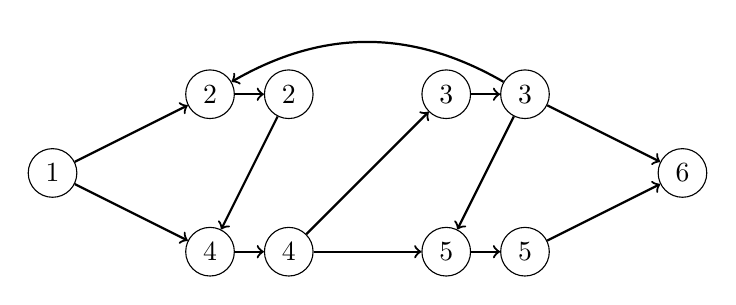
\begin{tikzpicture}
\node[draw, circle] (1) at (1,2) {$1$};

\node[draw, circle] (2a) at (3,3) {$2$};
\node[draw, circle] (3a) at (6,3) {$3$};
\node[draw, circle] (4a) at (3,1) {$4$};
\node[draw, circle] (5a) at (6,1) {$5$};

\node[draw, circle] (2b) at (4,3) {$2$};
\node[draw, circle] (3b) at (7,3) {$3$};
\node[draw, circle] (4b) at (4,1) {$4$};
\node[draw, circle] (5b) at (7,1) {$5$};

\node[draw, circle] (6) at (9,2) {$6$};

\path[draw,thick,->] (2a) -- (2b);
\path[draw,thick,->] (3a) -- (3b);
\path[draw,thick,->] (4a) -- (4b);
\path[draw,thick,->] (5a) -- (5b);

\path[draw,thick,->] (1) -- (2a);
\path[draw,thick,->] (1) -- (4a);
\path[draw,thick,->] (2b) -- (4a);
\path[draw,thick,->] (3b) edge [bend right=30] (2a);
\path[draw,thick,->] (3b) -- (5a);
\path[draw,thick,->] (3b) -- (6);
\path[draw,thick,->] (4b) -- (3a);
\path[draw,thick,->] (4b) -- (5a);
\path[draw,thick,->] (5b) -- (6);
\end{tikzpicture}
\end{center}

El flujo máximo para el gráfico es el siguiente:
\begin{center}
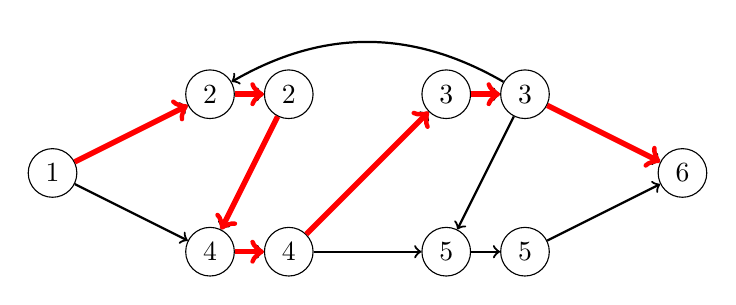
\begin{tikzpicture}
\node[draw, circle] (1) at (1,2) {$1$};

\node[draw, circle] (2a) at (3,3) {$2$};
\node[draw, circle] (3a) at (6,3) {$3$};
\node[draw, circle] (4a) at (3,1) {$4$};
\node[draw, circle] (5a) at (6,1) {$5$};

\node[draw, circle] (2b) at (4,3) {$2$};
\node[draw, circle] (3b) at (7,3) {$3$};
\node[draw, circle] (4b) at (4,1) {$4$};
\node[draw, circle] (5b) at (7,1) {$5$};

\node[draw, circle] (6) at (9,2) {$6$};

\path[draw,thick,->] (2a) -- (2b);
\path[draw,thick,->] (3a) -- (3b);
\path[draw,thick,->] (4a) -- (4b);
\path[draw,thick,->] (5a) -- (5b);

\path[draw,thick,->] (1) -- (2a);
\path[draw,thick,->] (1) -- (4a);
\path[draw,thick,->] (2b) -- (4a);
\path[draw,thick,->] (3b) edge [bend right=30] (2a);
\path[draw,thick,->] (3b) -- (5a);
\path[draw,thick,->] (3b) -- (6);
\path[draw,thick,->] (4b) -- (3a);
\path[draw,thick,->] (4b) -- (5a);
\path[draw,thick,->] (5b) -- (6);

\path[draw=red,thick,->,line width=2pt] (1) -- (2a);
\path[draw=red,thick,->,line width=2pt] (2a) -- (2b);
\path[draw=red,thick,->,line width=2pt] (2b) -- (4a);
\path[draw=red,thick,->,line width=2pt] (4a) -- (4b);
\path[draw=red,thick,->,line width=2pt] (4b) -- (3a);
\path[draw=red,thick,->,line width=2pt] (3a) -- (3b);
\path[draw=red,thick,->,line width=2pt] (3b) -- (6);
\end{tikzpicture}
\end{center}

Por lo tanto, el número máximo de caminos nodo-disjuntos
desde la fuente hasta el sumidero es 1.

\section{Emparejamientos máximos}

\index{emparejamiento}
\index{emparejamiento máximo}

El problema del \key{emparejamiento máximo} pide encontrar
un conjunto de tamaño máximo de pares de nodos en un grafo no dirigido
tal que cada par esté conectado con una arista y
cada nodo pertenezca a como máximo un par.

Existen algoritmos polinomiales para encontrar
emparejamientos máximos en grafos generales \cite{edm65},
pero tales algoritmos son complejos y
rara vez se ven en concursos de programación.
Sin embargo, en grafos bipartitos,
el problema del emparejamiento máximo es mucho más fácil
de resolver, porque podemos reducirlo al
problema de flujo máximo.

\subsubsection{Encontrar emparejamientos máximos}

Los nodos de un grafo bipartito siempre se pueden
dividir en dos grupos de modo que todas las aristas
del grafo vayan del grupo izquierdo al grupo derecho.
Por ejemplo, en el siguiente grafo bipartito,
los grupos son $\{1,2,3,4\}$ y $\{5,6,7,8\}$.

\begin{center}
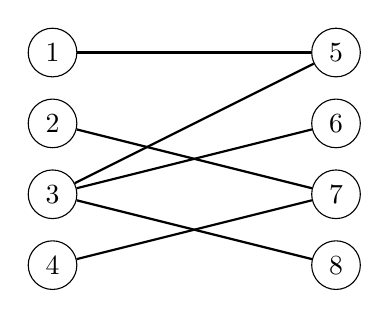
\begin{tikzpicture}[scale=0.60]
\node[draw, circle] (1) at (2,4.5) {1};
\node[draw, circle] (2) at (2,3) {2};
\node[draw, circle] (3) at (2,1.5) {3};
\node[draw, circle] (4) at (2,0) {4};
\node[draw, circle] (5) at (8,4.5) {5};
\node[draw, circle] (6) at (8,3) {6};
\node[draw, circle] (7) at (8,1.5) {7};
\node[draw, circle] (8) at (8,0) {8};

\path[draw,thick,-] (1) -- (5);
\path[draw,thick,-] (2) -- (7);
\path[draw,thick,-] (3) -- (5);
\path[draw,thick,-] (3) -- (6);
\path[draw,thick,-] (3) -- (8);
\path[draw,thick,-] (4) -- (7);
\end{tikzpicture}
\end{center}
El tamaño de un emparejamiento máximo de este grafo es 3:
\begin{center}
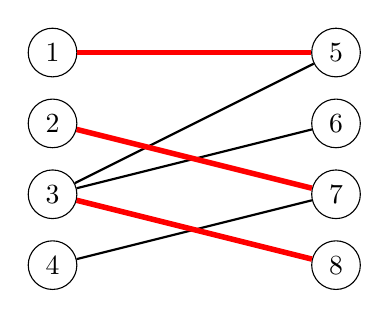
\begin{tikzpicture}[scale=0.60]
\node[draw, circle] (1) at (2,4.5) {1};
\node[draw, circle] (2) at (2,3) {2};
\node[draw, circle] (3) at (2,1.5) {3};
\node[draw, circle] (4) at (2,0) {4};
\node[draw, circle] (5) at (8,4.5) {5};
\node[draw, circle] (6) at (8,3) {6};
\node[draw, circle] (7) at (8,1.5) {7};
\node[draw, circle] (8) at (8,0) {8};

\path[draw,thick,-] (1) -- (5);
\path[draw,thick,-] (2) -- (7);
\path[draw,thick,-] (3) -- (5);
\path[draw,thick,-] (3) -- (6);
\path[draw,thick,-] (3) -- (8);
\path[draw,thick,-] (4) -- (7);

\path[draw=red,thick,-,line width=2pt] (1) -- (5);
\path[draw=red,thick,-,line width=2pt] (2) -- (7);
\path[draw=red,thick,-,line width=2pt] (3) -- (8);
\end{tikzpicture}
\end{center}

Podemos reducir el problema del emparejamiento máximo bipartito
al problema del flujo máximo agregando dos nuevos nodos
al grafo: una fuente y un sumidero.
También agregamos aristas desde la fuente
a cada nodo izquierdo y desde cada nodo derecho hasta el sumidero.
Después de esto, el tamaño de un flujo máximo en el grafo
es igual al tamaño de un emparejamiento máximo en el grafo original.

Por ejemplo, la reducción para el grafo anterior
es como sigue:
\begin{center}
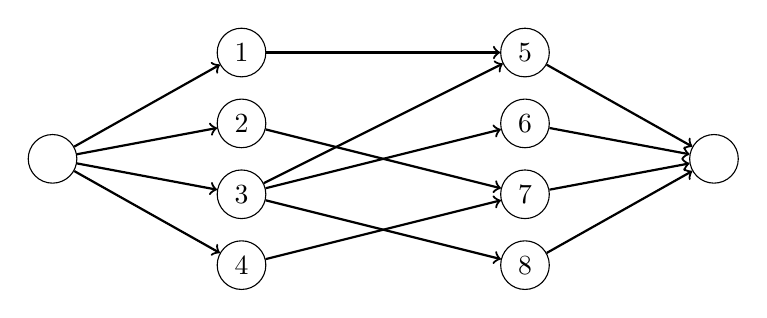
\begin{tikzpicture}[scale=0.60]
\node[draw, circle] (1) at (2,4.5) {1};
\node[draw, circle] (2) at (2,3) {2};
\node[draw, circle] (3) at (2,1.5) {3};
\node[draw, circle] (4) at (2,0) {4};
\node[draw, circle] (5) at (8,4.5) {5};
\node[draw, circle] (6) at (8,3) {6};
\node[draw, circle] (7) at (8,1.5) {7};
\node[draw, circle] (8) at (8,0) {8};

\node[draw, circle] (a) at (-2,2.25) {\phantom{0}};
\node[draw, circle] (b) at (12,2.25) {\phantom{0}};

\path[draw,thick,->] (1) -- (5);
\path[draw,thick,->] (2) -- (7);
\path[draw,thick,->] (3) -- (5);
\path[draw,thick,->] (3) -- (6);
\path[draw,thick,->] (3) -- (8);
\path[draw,thick,->] (4) -- (7);

\path[draw,thick,->] (a) -- (1);
\path[draw,thick,->] (a) -- (2);
\path[draw,thick,->] (a) -- (3);
\path[draw,thick,->] (a) -- (4);
\path[draw,thick,->] (5) -- (b);
\path[draw,thick,->] (6) -- (b);
\path[draw,thick,->] (7) -- (b);
\path[draw,thick,->] (8) -- (b);
\end{tikzpicture}
\end{center}

El flujo máximo de este grafo es como sigue:
\begin{center}
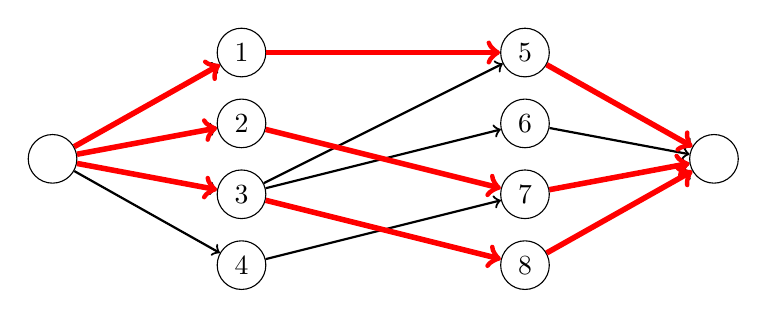
\begin{tikzpicture}[scale=0.60]
\node[draw, circle] (1) at (2,4.5) {1};
\node[draw, circle] (2) at (2,3) {2};
\node[draw, circle] (3) at (2,1.5) {3};
\node[draw, circle] (4) at (2,0) {4};
\node[draw, circle] (5) at (8,4.5) {5};
\node[draw, circle] (6) at (8,3) {6};
\node[draw, circle] (7) at (8,1.5) {7};
\node[draw, circle] (8) at (8,0) {8};

\node[draw, circle] (a) at (-2,2.25) {\phantom{0}};
\node[draw, circle] (b) at (12,2.25) {\phantom{0}};

\path[draw,thick,->] (3) -- (5);
\path[draw,thick,->] (3) -- (6);
\path[draw,thick,->] (4) -- (7);

\path[draw,thick,->] (a) -- (1);
\path[draw,thick,->] (a) -- (2);
\path[draw,thick,->] (a) -- (3);
\path[draw,thick,->] (a) -- (4);
\path[draw,thick,->] (5) -- (b);
\path[draw,thick,->] (6) -- (b);
\path[draw,thick,->] (7) -- (b);
\path[draw,thick,->] (8) -- (b);



\path[draw=red,thick,->,line width=2pt] (1) -- (5);
\path[draw=red,thick,->,line width=2pt] (2) -- (7);
\path[draw=red,thick,->,line width=2pt] (3) -- (8);

\path[draw=red,thick,->,line width=2pt] (a) -- (1);
\path[draw=red,thick,->,line width=2pt] (a) -- (2);
\path[draw=red,thick,->,line width=2pt] (a) -- (3);

\path[draw=red,thick,->,line width=2pt] (5) -- (b);
\path[draw=red,thick,->,line width=2pt] (7) -- (b);
\path[draw=red,thick,->,line width=2pt] (8) -- (b);

\end{tikzpicture}
\end{center}

\subsubsection{Teorema de Hall}

\index{Teorema de Hall}
\index{emparejamiento perfecto}

La \key{Teorema de Hall} se puede utilizar para averiguar
si un grafo bipartito tiene un emparejamiento
que contiene todos los nodos izquierdos o derechos.
Si el número de nodos izquierdos y derechos es el mismo,
el teorema de Hall nos dice si es posible
construir un \key{emparejamiento perfecto} que
contenga todos los nodos del grafo.

Supongamos que queremos encontrar un emparejamiento
que contenga todos los nodos izquierdos.
Sea $X$ cualquier conjunto de nodos izquierdos
y sea $f(X)$ el conjunto de sus vecinos.
De acuerdo con el teorema de Hall, un emparejamiento
que contiene todos los nodos izquierdos existe
exactamente cuando para cada $X$, la condición $|X| \le |f(X)|$ se cumple.

Estudiemos el teorema de Hall en el grafo de ejemplo.
Primero, sea $X=\{1,3\}$ lo que produce $f(X)=\{5,6,8\}$:

\begin{center}
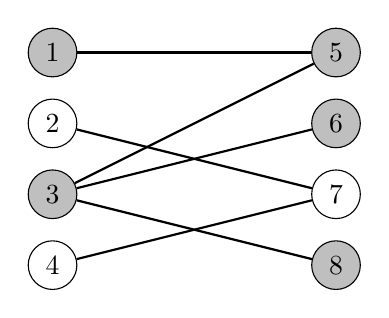
\begin{tikzpicture}[scale=0.60]
\node[draw, circle, fill=lightgray] (1) at (2,4.5) {1};
\node[draw, circle] (2) at (2,3) {2};
\node[draw, circle, fill=lightgray] (3) at (2,1.5) {3};
\node[draw, circle] (4) at (2,0) {4};
\node[draw, circle, fill=lightgray] (5) at (8,4.5) {5};
\node[draw, circle, fill=lightgray] (6) at (8,3) {6};
\node[draw, circle] (7) at (8,1.5) {7};
\node[draw, circle, fill=lightgray] (8) at (8,0) {8};

\path[draw,thick,-] (1) -- (5);
\path[draw,thick,-] (2) -- (7);
\path[draw,thick,-] (3) -- (5);
\path[draw,thick,-] (3) -- (6);
\path[draw,thick,-] (3) -- (8);
\path[draw,thick,-] (4) -- (7);
\end{tikzpicture}
\end{center}

La condición del teorema de Hall se cumple, porque
$|X|=2$ y $|f(X)|=3$.
Luego, sea $X=\{2,4\}$ lo que produce $f(X)=\{7\}$:

\begin{center}
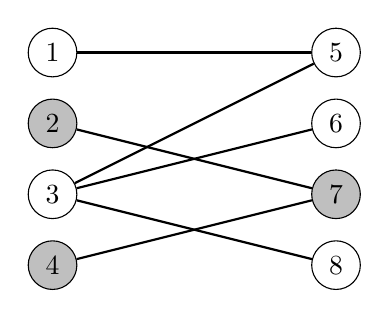
\begin{tikzpicture}[scale=0.60]
\node[draw, circle] (1) at (2,4.5) {1};
\node[draw, circle, fill=lightgray] (2) at (2,3) {2};
\node[draw, circle] (3) at (2,1.5) {3};
\node[draw, circle, fill=lightgray] (4) at (2,0) {4};
\node[draw, circle] (5) at (8,4.5) {5};
\node[draw, circle] (6) at (8,3) {6};
\node[draw, circle, fill=lightgray] (7) at (8,1.5) {7};
\node[draw, circle] (8) at (8,0) {8};

\path[draw,thick,-] (1) -- (5);
\path[draw,thick,-] (2) -- (7);
\path[draw,thick,-] (3) -- (5);
\path[draw,thick,-] (3) -- (6);
\path[draw,thick,-] (3) -- (8);
\path[draw,thick,-] (4) -- (7);
\end{tikzpicture}
\end{center}

En este caso, $|X|=2$ y $|f(X)|=1$,
por lo que la condición del teorema de Hall no se cumple.
Esto significa que no es posible formar
un emparejamiento perfecto para el grafo.
Este resultado no es sorprendente, porque ya
sabemos que el emparejamiento máximo del grafo es 3 y no 4.

Si la condición del teorema de Hall no se cumple,
el conjunto $X$ proporciona una explicación \emph{por qué}
no podemos formar tal emparejamiento.
Como $X$ contiene más nodos que $f(X)$,
no hay pares para todos los nodos en $X$.
Por ejemplo, en el grafo anterior, ambos nodos 2 y 4
deberían estar conectados con el nodo 7 lo cual no es posible.

\subsubsection{Teorema de Kőnig}

\index{Teorema de Kőnig}
\index{cubierta de nodos}
\index{cubierta de nodos mínima}

Una \key{cubierta de nodos mínima} de un grafo
es un conjunto mínimo de nodos tal que cada arista del grafo
tiene al menos un extremo en el conjunto.
En un grafo general, encontrar una cubierta de nodos mínima
es un problema NP-duro.
Sin embargo, si el grafo es bipartito,
el \key{Teorema de Kőnig} nos dice que
el tamaño de una cubierta de nodos mínima
y el tamaño de un emparejamiento máximo son siempre iguales.
Por lo tanto, podemos calcular el tamaño de una cubierta de nodos mínima
usando un algoritmo de flujo máximo.

Consideremos el siguiente grafo
con un emparejamiento máximo de tamaño 3:
\begin{center}
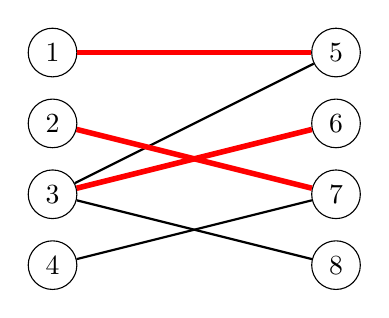
\begin{tikzpicture}[scale=0.60]
\node[draw, circle] (1) at (2,4.5) {1};
\node[draw, circle] (2) at (2,3) {2};
\node[draw, circle] (3) at (2,1.5) {3};
\node[draw, circle] (4) at (2,0) {4};
\node[draw, circle] (5) at (8,4.5) {5};
\node[draw, circle] (6) at (8,3) {6};
\node[draw, circle] (7) at (8,1.5) {7};
\node[draw, circle] (8) at (8,0) {8};

\path[draw,thick,-] (1) -- (5);
\path[draw,thick,-] (2) -- (7);
\path[draw,thick,-] (3) -- (5);
\path[draw,thick,-] (3) -- (6);
\path[draw,thick,-] (3) -- (8);
\path[draw,thick,-] (4) -- (7);

\path[draw=red,thick,-,line width=2pt] (1) -- (5);
\path[draw=red,thick,-,line width=2pt] (2) -- (7);
\path[draw=red,thick,-,line width=2pt] (3) -- (6);
\end{tikzpicture}
\end{center}
Ahora el teorema de Kőnig nos dice que el tamaño
de una cubierta de nodos mínima también es 3.
Tal cubierta se puede construir de la siguiente manera:

\begin{center}
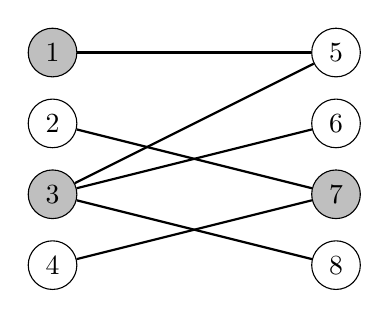
\begin{tikzpicture}[scale=0.60]
\node[draw, circle, fill=lightgray] (1) at (2,4.5) {1};
\node[draw, circle] (2) at (2,3) {2};
\node[draw, circle, fill=lightgray] (3) at (2,1.5) {3};
\node[draw, circle] (4) at (2,0) {4};
\node[draw, circle] (5) at (8,4.5) {5};
\node[draw, circle] (6) at (8,3) {6};
\node[draw, circle, fill=lightgray] (7) at (8,1.5) {7};
\node[draw, circle] (8) at (8,0) {8};

\path[draw,thick,-] (1) -- (5);
\path[draw,thick,-] (2) -- (7);
\path[draw,thick,-] (3) -- (5);
\path[draw,thick,-] (3) -- (6);
\path[draw,thick,-] (3) -- (8);
\path[draw,thick,-] (4) -- (7);
\end{tikzpicture}
\end{center}

\index{independent set}
\index{maximum independent set}

Los nodos que \emph{no}
pertenecen a una cobertura de nodos mínima
forman un conjunto \key{independiente máximo}.
Este es el conjunto más grande posible de nodos
tal que no hay dos nodos en el conjunto
conectados con una arista.
Una vez más, encontrar un conjunto independiente máximo
en un gráfico general es un problema NP-difícil,
pero en un gráfico bipartito podemos usar
el teorema de Kőnig para resolver el problema de manera eficiente.
En el gráfico de ejemplo, el conjunto independiente máximo
es el siguiente:

\begin{center}
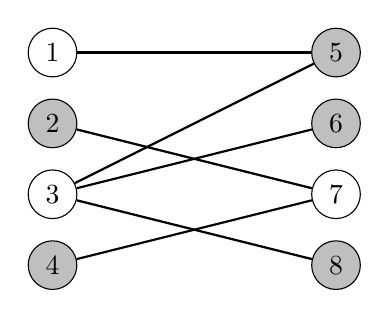
\begin{tikzpicture}[scale=0.60]
\node[draw, circle] (1) at (2,4.5) {1};
\node[draw, circle, fill=lightgray] (2) at (2,3) {2};
\node[draw, circle] (3) at (2,1.5) {3};
\node[draw, circle, fill=lightgray] (4) at (2,0) {4};
\node[draw, circle, fill=lightgray] (5) at (8,4.5) {5};
\node[draw, circle, fill=lightgray] (6) at (8,3) {6};
\node[draw, circle] (7) at (8,1.5) {7};
\node[draw, circle, fill=lightgray] (8) at (8,0) {8};

\path[draw,thick,-] (1) -- (5);
\path[draw,thick,-] (2) -- (7);
\path[draw,thick,-] (3) -- (5);
\path[draw,thick,-] (3) -- (6);
\path[draw,thick,-] (3) -- (8);
\path[draw,thick,-] (4) -- (7);
\end{tikzpicture}
\end{center}

\section{Coberturas de caminos}

\index{path cover}

Una \key{cobertura de caminos} es un conjunto de caminos en un gráfico
tal que cada nodo del gráfico pertenece a al menos un camino.
Resulta que en los gráficos dirigidos y acíclicos,
podemos reducir el problema de encontrar una cobertura de caminos mínima
al problema de encontrar un flujo máximo
en otro gráfico.

\subsubsection{Cobertura de caminos nodos-disjuntos}

En una \key{cobertura de caminos nodos-disjuntos},
cada nodo pertenece a exactamente un camino.
Como ejemplo, considera el siguiente gráfico:
\begin{center}
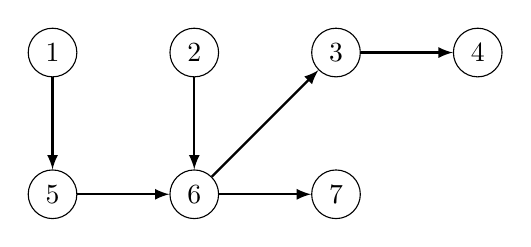
\begin{tikzpicture}[scale=0.9]
\node[draw, circle] (1) at (0,0) {1};
\node[draw, circle] (2) at (2,0) {2};
\node[draw, circle] (3) at (4,0) {3};
\node[draw, circle] (4) at (6,0) {4};
\node[draw, circle] (5) at (0,-2) {5};
\node[draw, circle] (6) at (2,-2) {6};
\node[draw, circle] (7) at (4,-2) {7};

\path[draw,thick,->,>=latex] (1) -- (5);
\path[draw,thick,->,>=latex] (2) -- (6);
\path[draw,thick,->,>=latex] (3) -- (4);
\path[draw,thick,->,>=latex] (5) -- (6);
\path[draw,thick,->,>=latex] (6) -- (3);
\path[draw,thick,->,>=latex] (6) -- (7);
\end{tikzpicture}
\end{center}

Una cobertura de caminos nodos-disjuntos mínima
de este gráfico
consta de tres caminos.
Por ejemplo, podemos elegir los siguientes caminos:

\begin{center}
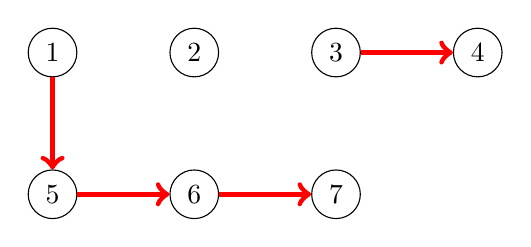
\begin{tikzpicture}[scale=0.9]
\node[draw, circle] (1) at (0,0) {1};
\node[draw, circle] (2) at (2,0) {2};
\node[draw, circle] (3) at (4,0) {3};
\node[draw, circle] (4) at (6,0) {4};
\node[draw, circle] (5) at (0,-2) {5};
\node[draw, circle] (6) at (2,-2) {6};
\node[draw, circle] (7) at (4,-2) {7};

\path[draw=red,thick,->,line width=2pt] (1) -- (5);
\path[draw=red,thick,->,line width=2pt] (5) -- (6);
\path[draw=red,thick,->,line width=2pt] (6) -- (7);
\path[draw=red,thick,->,line width=2pt] (3) -- (4);
\end{tikzpicture}
\end{center}

Tenga en cuenta que uno de los caminos solo contiene el nodo 2,
por lo que es posible que un camino no contenga ninguna arista.

Podemos encontrar una cobertura de caminos nodos-disjuntos mínima
construyendo un \emph{gráfico de coincidencia} donde cada nodo
del gráfico original está representado por
dos nodos: un nodo izquierdo y un nodo derecho.
Hay una arista de un nodo izquierdo a un nodo derecho
si hay una arista en el gráfico original.
Además, el gráfico de coincidencia contiene una fuente y un sumidero,
y hay aristas de la fuente a todos
los nodos izquierdos y de todos los nodos derechos al sumidero.

Una coincidencia máxima en el gráfico resultante corresponde
a una cobertura de caminos nodos-disjuntos mínima en
el gráfico original.
Por ejemplo, el siguiente gráfico de coincidencia
para el gráfico anterior contiene
una coincidencia máxima de tamaño 4:

\begin{center}
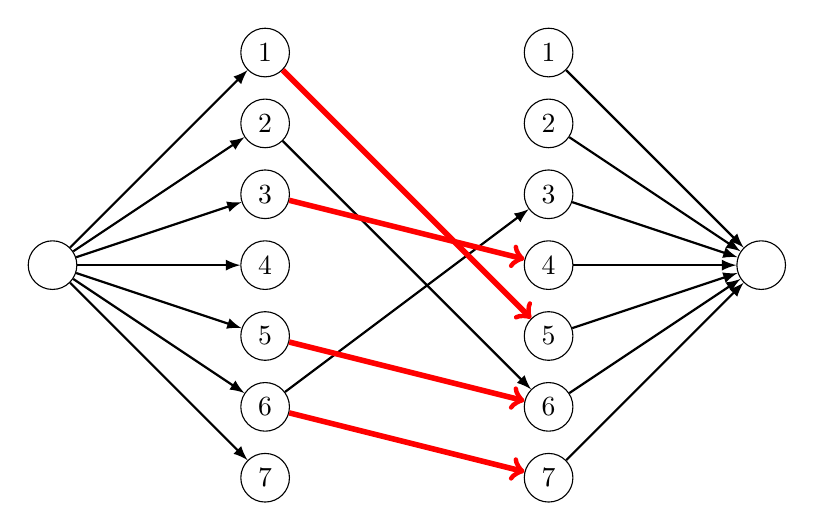
\begin{tikzpicture}[scale=0.9]
\node[draw, circle] (1a) at (0,6) {1};
\node[draw, circle] (2a) at (0,5) {2};
\node[draw, circle] (3a) at (0,4) {3};
\node[draw, circle] (4a) at (0,3) {4};
\node[draw, circle] (5a) at (0,2) {5};
\node[draw, circle] (6a) at (0,1) {6};
\node[draw, circle] (7a) at (0,0) {7};

\node[draw, circle] (1b) at (4,6) {1};
\node[draw, circle] (2b) at (4,5) {2};
\node[draw, circle] (3b) at (4,4) {3};
\node[draw, circle] (4b) at (4,3) {4};
\node[draw, circle] (5b) at (4,2) {5};
\node[draw, circle] (6b) at (4,1) {6};
\node[draw, circle] (7b) at (4,0) {7};

\node[draw, circle] (a) at (-3,3) {\phantom{0}};
\node[draw, circle] (b) at (7,3) {\phantom{0}};

%\path[draw,thick,->,>=latex] (1a) -- (5b);
\path[draw,thick,->,>=latex] (2a) -- (6b);
%\path[draw,thick,->,>=latex] (3a) -- (4b);
%\path[draw,thick,->,>=latex] (5a) -- (6b);
\path[draw,thick,->,>=latex] (6a) -- (3b);
%\path[draw,thick,->,>=latex] (6a) -- (7b);

\path[draw,thick,->,>=latex] (a) -- (1a);
\path[draw,thick,->,>=latex] (a) -- (2a);
\path[draw,thick,->,>=latex] (a) -- (3a);
\path[draw,thick,->,>=latex] (a) -- (4a);
\path[draw,thick,->,>=latex] (a) -- (5a);
\path[draw,thick,->,>=latex] (a) -- (6a);
\path[draw,thick,->,>=latex] (a) -- (7a);

\path[draw,thick,->,>=latex] (1b) -- (b);
\path[draw,thick,->,>=latex] (2b) -- (b);
\path[draw,thick,->,>=latex] (3b) -- (b);
\path[draw,thick,->,>=latex] (4b) -- (b);
\path[draw,thick,->,>=latex] (5b) -- (b);
\path[draw,thick,->,>=latex] (6b) -- (b);
\path[draw,thick,->,>=latex] (7b) -- (b);

\path[draw=red,thick,->,line width=2pt] (1a) -- (5b);
\path[draw=red,thick,->,line width=2pt] (5a) -- (6b);
\path[draw=red,thick,->,line width=2pt] (6a) -- (7b);
\path[draw=red,thick,->,line width=2pt] (3a) -- (4b);

\end{tikzpicture}
\end{center}

Cada arista en la coincidencia máxima del gráfico de coincidencia corresponde
a una arista en la cubierta mínima de camino sin nodos coincidentes
del gráfico original.
Por lo tanto, el tamaño de la cubierta mínima de camino sin nodos coincidentes es $n-c$,
donde $n$ es el número de nodos en el gráfico original
y $c$ es el tamaño de la coincidencia máxima.

\subsubsection{Cubierta general de caminos}

Una \key{cubierta general de caminos} es una cubierta de caminos
donde un nodo puede pertenecer a más de un camino.
Una cubierta general de caminos mínima puede ser más pequeña
que una cubierta mínima de camino sin nodos coincidentes,
porque un nodo puede utilizarse varias veces en caminos.
Considere nuevamente el siguiente gráfico:
\begin{center}
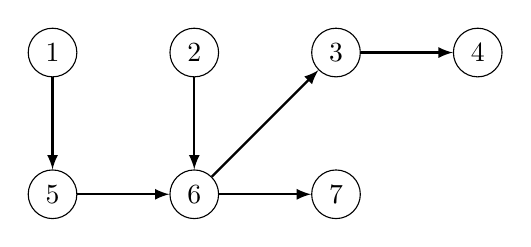
\begin{tikzpicture}[scale=0.9]
\node[draw, circle] (1) at (0,0) {1};
\node[draw, circle] (2) at (2,0) {2};
\node[draw, circle] (3) at (4,0) {3};
\node[draw, circle] (4) at (6,0) {4};
\node[draw, circle] (5) at (0,-2) {5};
\node[draw, circle] (6) at (2,-2) {6};
\node[draw, circle] (7) at (4,-2) {7};

\path[draw,thick,->,>=latex] (1) -- (5);
\path[draw,thick,->,>=latex] (2) -- (6);
\path[draw,thick,->,>=latex] (3) -- (4);
\path[draw,thick,->,>=latex] (5) -- (6);
\path[draw,thick,->,>=latex] (6) -- (3);
\path[draw,thick,->,>=latex] (6) -- (7);
\end{tikzpicture}
\end{center}

La cubierta general de caminos mínima de este gráfico
consiste en dos caminos.
Por ejemplo, el primer camino puede ser el siguiente:
\begin{center}
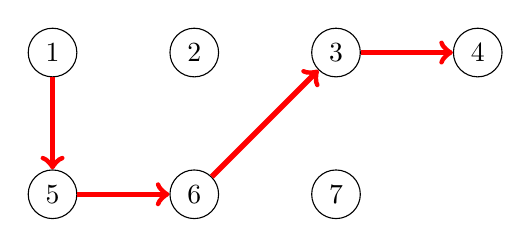
\begin{tikzpicture}[scale=0.9]
\node[draw, circle] (1) at (0,0) {1};
\node[draw, circle] (2) at (2,0) {2};
\node[draw, circle] (3) at (4,0) {3};
\node[draw, circle] (4) at (6,0) {4};
\node[draw, circle] (5) at (0,-2) {5};
\node[draw, circle] (6) at (2,-2) {6};
\node[draw, circle] (7) at (4,-2) {7};

\path[draw=red,thick,->,line width=2pt] (1) -- (5);
\path[draw=red,thick,->,line width=2pt] (5) -- (6);
\path[draw=red,thick,->,line width=2pt] (6) -- (3);
\path[draw=red,thick,->,line width=2pt] (3) -- (4);
\end{tikzpicture}
\end{center}
Y el segundo camino puede ser el siguiente:
\begin{center}
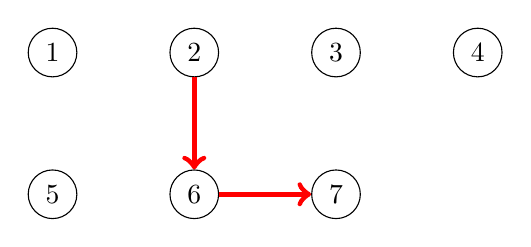
\begin{tikzpicture}[scale=0.9]
\node[draw, circle] (1) at (0,0) {1};
\node[draw, circle] (2) at (2,0) {2};
\node[draw, circle] (3) at (4,0) {3};
\node[draw, circle] (4) at (6,0) {4};
\node[draw, circle] (5) at (0,-2) {5};
\node[draw, circle] (6) at (2,-2) {6};
\node[draw, circle] (7) at (4,-2) {7};

\path[draw=red,thick,->,line width=2pt] (2) -- (6);
\path[draw=red,thick,->,line width=2pt] (6) -- (7);
\end{tikzpicture}
\end{center}

Una cubierta general de caminos mínima puede encontrarse
casi como una cubierta mínima de camino sin nodos coincidentes.
Basta con agregar algunas aristas nuevas al gráfico de coincidencia
para que haya una arista $a \rightarrow b$
siempre cuando haya un camino de $a$ a $b$
en el gráfico original (posiblemente a través de varias aristas).

El gráfico de coincidencia para el gráfico anterior es el siguiente:
\begin{center}
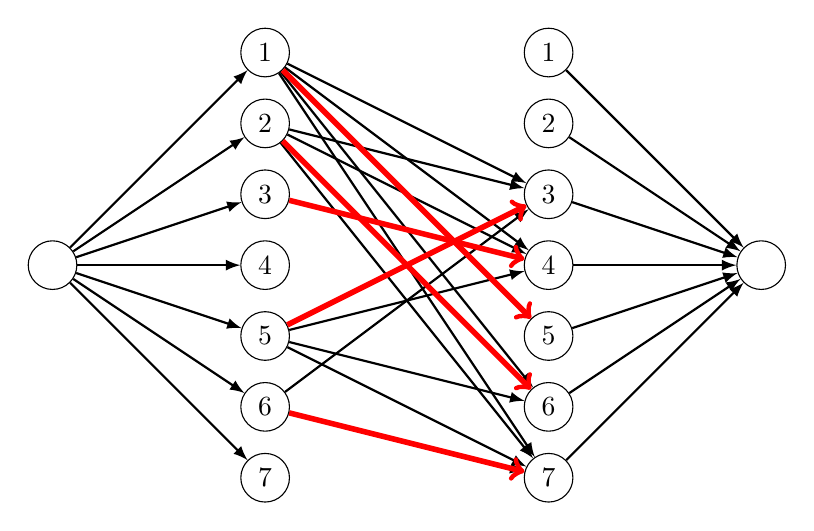
\begin{tikzpicture}[scale=0.9]
\node[draw, circle] (1a) at (0,6) {1};
\node[draw, circle] (2a) at (0,5) {2};
\node[draw, circle] (3a) at (0,4) {3};
\node[draw, circle] (4a) at (0,3) {4};
\node[draw, circle] (5a) at (0,2) {5};
\node[draw, circle] (6a) at (0,1) {6};
\node[draw, circle] (7a) at (0,0) {7};

\node[draw, circle] (1b) at (4,6) {1};
\node[draw, circle] (2b) at (4,5) {2};
\node[draw, circle] (3b) at (4,4) {3};
\node[draw, circle] (4b) at (4,3) {4};
\node[draw, circle] (5b) at (4,2) {5};
\node[draw, circle] (6b) at (4,1) {6};
\node[draw, circle] (7b) at (4,0) {7};

\node[draw, circle] (a) at (-3,3) {\phantom{0}};
\node[draw, circle] (b) at (7,3) {\phantom{0}};


%\path[draw,thick,->,>=latex] (1a) -- (5b);
\path[draw,thick,->,>=latex] (1a) -- (6b);
\path[draw,thick,->,>=latex] (1a) -- (7b);
\path[draw,thick,->,>=latex] (1a) -- (3b);
\path[draw,thick,->,>=latex] (1a) -- (4b);
\path[draw,thick,->,>=latex] (5a) -- (6b);
\path[draw,thick,->,>=latex] (5a) -- (7b);
%\path[draw,thick,->,>=latex] (5a) -- (3b);
\path[draw,thick,->,>=latex] (5a) -- (4b);
\path[draw,thick,->,>=latex] (6a) -- (7b);
%\path[draw,thick,->,>=latex] (6a) -- (7b);
\path[draw,thick,->,>=latex] (6a) -- (3b);
%\path[draw,thick,->,>=latex] (3a) -- (4b);
%\path[draw,thick,->,>=latex] (2a) -- (6b);
\path[draw,thick,->,>=latex] (2a) -- (7b);
\path[draw,thick,->,>=latex] (2a) -- (3b);
\path[draw,thick,->,>=latex] (2a) -- (4b);


\path[draw,thick,->,>=latex] (a) -- (1a);
\path[draw,thick,->,>=latex] (a) -- (2a);
\path[draw,thick,->,>=latex] (a) -- (3a);
\path[draw,thick,->,>=latex] (a) -- (4a);
\path[draw,thick,->,>=latex] (a) -- (5a);
\path[draw,thick,->,>=latex] (a) -- (6a);
\path[draw,thick,->,>=latex] (a) -- (7a);

\path[draw,thick,->,>=latex] (1b) -- (b);
\path[draw,thick,->,>=latex] (2b) -- (b);
\path[draw,thick,->,>=latex] (3b) -- (b);
\path[draw,thick,->,>=latex] (4b) -- (b);
\path[draw,thick,->,>=latex] (5b) -- (b);
\path[draw,thick,->,>=latex] (6b) -- (b);
\path[draw,thick,->,>=latex] (7b) -- (b);

\path[draw=red,thick,->,line width=2pt] (1a) -- (5b);
\path[draw=red,thick,->,line width=2pt] (5a) -- (3b);
\path[draw=red,thick,->,line width=2pt] (3a) -- (4b);
\path[draw=red,thick,->,line width=2pt] (2a) -- (6b);
\path[draw=red,thick,->,line width=2pt] (6a) -- (7b);


% \path[draw=red,thick,->,line width=2pt] (1a) -- (6b);
% \path[draw=red,thick,->,line width=2pt] (1a) -- (7b);
% \path[draw=red,thick,->,line width=2pt] (1a) -- (3b);
% \path[draw=red,thick,->,line width=2pt] (1a) -- (4b);
% \path[draw=red,thick,->,line width=2pt] (5a) -- (6b);
% \path[draw=red,thick,->,line width=2pt] (5a) -- (7b);
% \path[draw=red,thick,->,line width=2pt] (5a) -- (3b);
% \path[draw=red,thick,->,line width=2pt] (5a) -- (4b);
% \path[draw=red,thick,->,line width=2pt] (6a) -- (7b);
% \path[draw=red,thick,->,line width=2pt] (6a) -- (7b);
% \path[draw=red,thick,->,line width=2pt] (6a) -- (3b);
% \path[draw=red,thick,->,line width=2pt] (3a) -- (4b);
% \path[draw=red,thick,->,line width=2pt] (2a) -- (6b);
% \path[draw=red,thick,->,line width=2pt] (2a) -- (7b);
% \path[draw=red,thick,->,line width=2pt] (2a) -- (3b);
% \path[draw=red,thick,->,line width=2pt] (2a) -- (4b);

\end{tikzpicture}
\end{center}

\subsubsection{Teorema de Dilworth}

\index{Teorema de Dilworth}
\index{cadena}

Una \key{cadena} es un conjunto de nodos de un grafo
tal que no hay camino
desde ningún nodo a otro nodo
usando las aristas del grafo.
El \key{Teorema de Dilworth} establece que
en un grafo acíclico dirigido, el tamaño de
una cubierta de camino general mínima
es igual al tamaño de una cadena máxima.

Por ejemplo, los nodos 3 y 7 forman una cadena
en el siguiente grafo:

\begin{center}
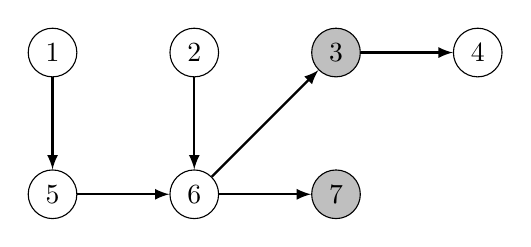
\begin{tikzpicture}[scale=0.9]
\node[draw, circle] (1) at (0,0) {1};
\node[draw, circle] (2) at (2,0) {2};
\node[draw, circle, fill=lightgray] (3) at (4,0) {3};
\node[draw, circle] (4) at (6,0) {4};
\node[draw, circle] (5) at (0,-2) {5};
\node[draw, circle] (6) at (2,-2) {6};
\node[draw, circle, fill=lightgray] (7) at (4,-2) {7};

\path[draw,thick,->,>=latex] (1) -- (5);
\path[draw,thick,->,>=latex] (2) -- (6);
\path[draw,thick,->,>=latex] (3) -- (4);
\path[draw,thick,->,>=latex] (5) -- (6);
\path[draw,thick,->,>=latex] (6) -- (3);
\path[draw,thick,->,>=latex] (6) -- (7);
\end{tikzpicture}
\end{center}

Esta es una cadena máxima, porque no es posible
construir ninguna cadena que contenga tres nodos.
Hemos visto antes que el tamaño de una
cubierta de camino general mínima de este grafo consiste en dos caminos.
